\id{МРНТИ: 06.71.57}{https://doi.org/10.58805/kazutb.v.2.27-1055}

\begin{articleheader}
\sectionwithauthors{М.Б.Идрышов}{GOOGLE TRENDS ҚҰРАЛЫН ПАЙДАЛАНЫП, ҚАЗАҚСТАННЫҢ ТУРИСТІК БАҒЫТТАРЫНА ЦИФРЛЫҚ ҚЫЗЫҒУШЫЛЫҚТЫ ТАЛДАУ}

{\bfseries
М.Б.Идрышов\alink{https://orcid.org/0009-0006-9509-6229}
}
\end{articleheader}

\begin{affiliation}
С. Аманжолов атындағы Шығыс Қазақстан университеті, Өскемен Қазақстан

\raggedright \textsuperscript{\envelope }Корреспондент-автор: immakhambet@gmail.com
\end{affiliation}

Осы мақала Қазақстан Республикасындағы туристік бағыттарға деген цифрлық
қызығушылықты Google Trends платформасының деректері негізінде талдауға
арналған. Туризм бойынша өзекті өңірлік статистиканың шектеулі болуына
байланысты пайдаланушылардың цифрлық іздерін қолдану мінез-құлықтық
үрдістерді бақылау мен талдаудың маңызды құралына айналуда. Зерттеудің
мақсаты -- Алматы, Астана және Қазақстан бойынша негізгі бағыттарға
деген қызығушылықты бағалау, сондай-ақ орыс және ағылшын тілдеріндегі
сұраныс құрылымының ерекшеліктерін ескере отырып, Google Trends қолдану
мүмкіндігін зерттеу. Зерттеу аясында туристік сұранысты бейнелейтін 240
сұраныстан тұратын дерекқор жасалды. Талдаудың сенімділігін арттыру үшін
деректер екі кезеңде (2016--2022 және 2022--2025) жиналып, біртекті
шкалаға келтіріліп, агрегацияланды. Корреляциялық талдау нәтижесінде (r
≥ 0.3) тұрақты сұраныстар іріктеліп, әрбір бағыт пен тілдік топ бойынша
қызығушылық индекстері жасалды. Талдау нәтижесінде ағылшын тіліндегі
сұраныстардың басым бөлігі логистикаға (ұшақ билеттері, рейстер) қатысты
екенін, ал орыс тіліндегі сұраныстарда туристік орындар мен қалалық
инфрақұрылым элементтерінің атаулары жиі кездесетінін көрсетті. Бұл ішкі
және халықаралық туризм арасындағы айырмашылықтарды, сондай-ақ ағылшын
тілді пайдаланушылар арасында іскерлік сапарлардың басымдығын көрсетуі
мүмкін. Зерттеу нәтижелері әдістемелік бейімделу жағдайында Google
Trends құралын туристік сұранысты талдау құралы ретінде қолдануға
болатындығын растады. Бұл жұмыс бағыттар бойынша қызығушылықтың
мінез-құлықтық ерекшеліктерін көрсетіп, Қазақстанда туризмді дамыту
стратегиясын қолдау үшін цифрлық деректерді пайдаланудың келешегін атап
өтеді.

{\bfseries Түйін сөздер}: Google Trends, цифрлық із, туристік сұраныс,
агрегатталған қызығушылық индексі, корреляциялық талдау, Қазақстан, ішкі
туризм, іскерлік туризм.

\begin{articleheader}
{\bfseries АНАЛИЗ ЦИФРОВОГО ИНТЕРЕСА К ТУРИСТИЧЕСКИМ НАПРАВЛЕНИЯМ КАЗАХСТАНА С ИСПОЛЬЗОВАНИЕМ GOOGLE TRENDS}

{\bfseries М.Б.Идрышов}
\end{articleheader}

\begin{affiliation}
НАО «Восточно-Казахстанский университет им. С. Аманжолова», Усть-Каменогорск, Казахстан,

e-mail: immakhambet@gmail.com
\end{affiliation}

Настоящая статья посвящена анализу цифрового интереса к туристическим
направлениям Республики Казахстан на основе данных платформы Google
Trends. В условиях ограниченной доступности актуальной региональной
статистики по туризму использование цифровых следов пользователей
становится важным инструментом для мониторинга и анализа поведенческих
тенденций. Целью исследования является оценка применимости Google Trends
для анализа интереса к ключевым направлениям --- Алматы, Астана и
Казахстан в целом --- с учётом различий между русскоязычным и
англоязычным сегментами. В рамках работы была сформирована база из 240
поисковых запросов на русском и английском языках, отражающих интерес к
туристическим поездкам. Для повышения достоверности анализа данные были
собраны за два периода (2016--2022 и 2022--2025), приведены к единому
масштабу и агрегированы. Далее с использованием корреляционного анализа
были отобраны стабильные запросы (r ≥ 0.3), по которым сформированы
индексы интереса к каждому направлению и языковой группе. Итоговый
анализ показал, что подавляющее большинство англоязычных запросов
касаются логистики (авиабилеты, перелёты), тогда как в русскоязычном
сегменте преобладают названия конкретных достопримечательностей и
элементов городской инфраструктуры. Это может указывать на различия
между внутренним и международным типами туризма, а также на
потенциальное преобладание деловых поездок среди англоязычных
пользователей. Полученные результаты подтверждают применимость Google
Trends как инструмента анализа туристического спроса при условии
корректной методической адаптации. Исследование выявляет поведенческие
особенности интереса к разным направлениям и подчёркивает
перспективность использования цифровых данных для поддержки стратегий
развития туризма в Казахстане.

{\bfseries Ключевые слова}: Google Trends, цифровой след, туристический
спрос, агрегированный индекс интереса, корреляционный анализ, Казахстан,
внутренний туризм, деловой туризм.

\begin{articleheader}
{\bfseries ANALYSIS OF DIGITAL INTEREST IN TOURIST DESTINATIONS OF KAZAKHSTAN USING GOOGLE TRENDS}

{\bfseries M.B.Idryshov}
\end{articleheader}

\begin{affiliation}
S. Amanzholov East Kazakhstan University, Ust-Kamenogorsk, Kazakhstan,

e-mail: immakhambet@gmail.com
\end{affiliation}

This article explores digital interest in tourist destinations in the
Republic of Kazakhstan using data from the Google Trends platform. In
the context of limited availability of up-to-date regional tourism
statistics, the use of users' digital traces becomes an important tool
for monitoring and analyzing behavioral patterns. The objective of the
study is to assess the applicability of Google Trends for analyzing
interest in key destinations---Almaty, Astana, and Kazakhstan as a
whole---considering differences between Russian-speaking and
English-speaking user segments. A dataset of 240 search queries in
Russian and English related to tourism was compiled. To ensure the
reliability of the analysis, data were collected across two periods
(2016--2022 and 2022--2025), normalized, and aggregated. Based on
correlation analysis (r ≥ 0.3), stable queries were selected and used to
construct interest indices for each destination and language group. The
final analysis revealed that most English-language queries related to
logistics (flights, travel), while the Russian-language queries mostly
referenced specific tourist sites and elements of urban infrastructure.
This may indicate differences between domestic and international tourism
patterns and possibly a dominance of business travel among
English-speaking users. The findings confirm the applicability of Google
Trends as a tool for analyzing tourism demand, provided that the
methodology is carefully adapted. The study highlights behavioral
specifics in destination interest and emphasizes the potential of
digital data to support tourism development strategies in Kazakhstan.

{\bfseries Keywords}: Google Trends, digital trace, tourism demand,
aggregated interest index, correlation analysis, Kazakhstan, domestic
tourism,business tourism.

\begin{multicols}{2}
{\bfseries Введение.} В последние годы наблюдается стремительный рост
интереса к использованию больших данных в социально-экономических
исследованиях. Одним из наиболее доступных и оперативных инструментов
анализа пользовательского поведения выступает Google Trends - платформа,
позволяющая отслеживать частотность поисковых запросов пользователей по
различным темам. Это особенно актуально в условиях, когда традиционная
туристическая статистика доступна с существенной временной задержкой, а
поведение потребителей всё чаще начинает формироваться онлайн.

Несмотря на возрастающий интерес к цифровым источникам данных, их
использование в академических и прикладных исследованиях в Казахстане
остаётся фрагментарным. Между тем, в международной практике Google
Trends активно используется для прогнозирования туристического спроса
как на национальном, так и на региональном уровне {[}1, 2{]}.

Подобные подходы начали применяться и в исследованиях на постсоветском
пространстве. В частности, в России Google Trends использовался для
анализа ментальных связей между регионами {[}3{]}, политических
настроений {[}4{]}, а также как инструмент веб-аналитики в прикладных
социологических и маркетинговых работах {[}5{]}. Однако в туризме
подобные исследования носят единичный характер и практически не касаются
стран Центральной Азии, включая Казахстан, что подчёркивает научную
новизну данного исследования.

При этом научное сообщество указывает на ряд методологических трудностей
при работе с данными Google Trends - от ограниченного временного охвата
и нормализации значений до необходимости корректной агрегации запросов и
сглаживания сезонных искажающих эффектов {[}6{]}. Эти аспекты требуют
критического подхода к интерпретации результатов и подчёркивают
необходимость адаптации методик к региональной специфике.

Настоящее исследование фокусируется на интересе пользователей к
туристическим направлениям Казахстана, таким как Астана, Алматы и страна
в целом, с учётом языковой специфики запросов (русский и английский).
Такой подход позволяет учесть как внутренний, так и потенциальный
въездной туризм, зафиксированный в цифровом поведении пользователей.

Выбор темы исследования обусловлен необходимостью изучения новых
подходов к анализу туристического спроса в Республике Казахстан,
основанных на цифровых следах поведения пользователей. Несмотря на
активное применение Google Trends в прогнозировании экономических
индикаторов, таких как уровень безработицы, инфляция и потребительские
настроения, его использование в сфере туризма, особенно в казахстанском
контексте, всё ещё ограничено {[}7{]}.

Актуальность темы подтверждается глобальной тенденцией цифровизации
туристической отрасли, ростом числа онлайн-бронирований и поисковых
запросов, отражающих намерения потенциальных туристов. Исследования
показывают, что интерес к направлениям, выраженный через поисковые
запросы, может выступать в качестве опережающего индикатора
туристических потоков {[}7{]}. В условиях Казахстана, где официальная
статистика по регионам может быть ограниченной, такой подход особенно
ценен.

Объект исследования - туристический спрос в Республике Казахстан.\\
Предмет исследования - поисковая активность в Google как индикатор
интереса к туристическим направлениям.

Цель исследования - определить потенциал использования данных Google
Trends для анализа и прогнозирования интереса к различным туристическим
направлениям в Казахстане.

Задачи исследования:


1. Провести сбор и агрегацию поисковых данных по ключевым туристическим
направлениям;

2. Выделить наиболее популярные запросы и проанализировать их сезонную и
географическую структуру;

3. Провести корреляционный анализ между поисковыми запросами;

4. Выявить ограничения и методические риски при использовании Google
Trends в региональных исследованиях.

Гипотеза исследования заключается в том, что поисковые запросы
пользователей в Google Trends демонстрируют устойчивые и повторяющиеся
сезонные паттерны интереса к туристическим направлениям в Казахстане.
Отдельной целью исследования выступает оценка применимости Google Trends
как инструмента анализа интереса к туристическим направлениям в условиях
Казахстана.

Научная и практическая значимость исследования проявляется в применении
цифровых следов пользователей к анализу туристического спроса на уровне
страны, что особенно важно в условиях ограниченной доступности
оперативной официальной статистики.

{\bfseries Материалы и методы.} Настоящее исследование направлено на
выявление потенциала использования поисковой активности пользователей в
Google как индикатора туристического спроса в Республике Казахстан.
Вопрос исследования заключается в следующем: может ли частотность
поисковых запросов, зафиксированная в сервисе Google Trends, служить
надёжной основой для анализа поведенческих тенденций, связанных с
туристической активностью? Исходная гипотеза предполагает, что
существует устойчивая взаимосвязь между цифровыми следами интереса к
направлениям и реальным туристическим спросом, особенно в условиях
ограниченной детализации официальной статистики.

В качестве исследовательского материала использовались данные поисковых
запросов, выгруженные из Google Trends. Были выбраны три ключевых
направления --- Астана, Алматы и Казахстан в целом, а также включено
отдельное направление «Нур-Султан» как промежуточное название столицы.
Для каждого направления сформированы по 30 запросов на русском и
английском языках, что в сумме дало 240 уникальных поисковых фраз. Все
выгрузки проводились с использованием встроенной категории Google Trends
«Путешествия», что обеспечило тематическую фильтрацию данных и исключило
нерелевантные значения {[}8{]}. География запросов была установлена как
"по всему миру", поскольку целью являлось выявление совокупного интереса
к туристическим направлениям в Казахстане как со стороны внутренних, так
и внешних пользователей.

При формировании набора поисковых фраз в исследование были включены
только запросы на русском и английском языках. Это объясняется тем, что
география выгрузки в Google Trends была установлена как «по всему миру»,
а русскоязычные и англоязычные формулировки обладают более широкой
распространённостью и, как следствие, большей частотностью использования
среди как внутренних, так и внешних пользователей. Поскольку казахский
язык не является глобально распространённым и встречается значительно
реже в открытом поисковом поведении, было принято решение не включать
его на данном этапе анализа. Тем не менее, использование казахоязычных
запросов может представлять интерес для локализованных будущих
исследований с фокусом на внутри казахстанскую выборку.

Сами поисковые фразы были сформированы относительно рандомизированным
образом с использованием возможностей языковой модели ChatGPT,
выступающей в роли генератора вариантов на русском и английском языках
по каждому направлению. Генерация базировалась на тематических
подсказках (например, "Алматы отдых", "Kazakhstan tour",
"достопримечательности Астаны" и др.) и последующей автоматической
вариативности модели. Далее полученные предложения подвергались ручной
проверке и отбору с целью исключения неинформативных, повторяющихся или
нерелевантных конструкций.

В связи с особенностями алгоритмов Google Trends, изменявшихся в 2016 и
2021 годах, данные собирались по двум временным периодам: с 1 января
2016 года по 31 декабря 2022 года и с 1 января 2022 года по 11 мая 2025
года {[}9{]}. Первый период представлен в формате месячных значений,
второй - в недельном. Чтобы обеспечить возможность объединения этих
периодов в непрерывный временной ряд, год 2022 был включён в оба периода
в качестве перекрытия. Такое решение позволило рассчитать коэффициенты
пересчёта между периодами на основе сопоставимых участков данных.

Для минимизации эффекта случайности, связанного с особенностями выдачи
Google Trends, по каждому запросу в каждом периоде было выполнено по три
выгрузки. Далее для каждого месяца вычислялось среднее значение, что
позволило стабилизировать ряды {[}7{]}. Для второго периода,
представленного в недельном формате, применялась агрегация на уровне
месяца путём усреднения всех недель, начинающихся в пределах
соответствующего месяца {[}10{]}.

Поскольку данные Google Trends нормализованы внутри каждой выгрузки
(максимум = 100), для приведения значений двух периодов к единой шкале
по каждому запросу отдельно рассчитывался коэффициент пересчёта: среднее
значение за первый период делилось на среднее значение за второй. Далее
все значения второго периода умножались на этот коэффициент, в
результате чего значения приобретали сопоставимость с первым периодом.
Такой подход соответствует методике, предложенной France \& Shi {[}6{]},
и позволяет устранять искажения, возникающие из-за внутренней
нормализации данных в Google Trends.

После пересчёта и агрегирования все данные были объединены в единый
временной ряд по каждому из запросов, охватывающий период с января 2016
года по апрель 2025 года. Недели мая, включённые в последнюю выгрузку,
не учитывались, поскольку на момент сбора данных были доступны только
первые две недели месяца, что не позволяло корректно сформировать полное
месячное значение.

На следующем этапе был проведён корреляционный анализ Пирсона между
временными рядами внутри каждой тематической подгруппы, определяемой
направлением (Астана, Алматы, Казахстан) и языком запроса (русский,
английский). Целью анализа являлась оценка степени согласованности
поведения запросов, относящихся к одному направлению, но отличающихся по
формулировке. Запросы, демонстрировавшие низкий уровень взаимной
корреляции (r ≤ 0.3) с остальными в подгруппе, исключались из
дальнейшего анализа как нестабильные или нерепрезентативные {[}1{]}.

Оставшиеся согласованные запросы использовались для построения
агрегированных индексов интереса по каждому направлению и языковой
группе. Индексы формировались путём усреднения нормализованных значений
по каждому месяцу и отражали общий поведенческий интерес к
соответствующему направлению. Такой подход позволил сгладить
индивидуальные колебания по отдельным запросам и обеспечить
репрезентативность итогового показателя интереса, соответствуя методике,
рекомендованной France \& Shi {[}6{]}.

Таким образом, совокупность методических решений в исследовании
направлена на повышение достоверности результатов анализа и адаптацию
международных практик к специфике цифрового поведения в туристической
сфере Казахстана.

{\bfseries Обсуждение и результаты.} Проведённый анализ показал, что из 240
поисковых запросов (табл.1), сформированных по трём основным
туристическим направлениям в Казахстане (Астана, Алматы, Казахстан в
целом), только 21 запрос (табл.2) соответствовал критериям стабильности
и содержательной релевантности. Остальные были исключены из-за высокой
нестабильности значений между периодами, выраженных скачков, отсутствия
повторяемости или избыточной фрагментарности данных. Это подтверждает
ограниченность универсального применения Google Trends в регионах с
меньшей плотностью запросов и подчёркивает необходимость индивидуального
отбора и валидации терминов, как это также отмечается в работе Önder
{[}7{]} и France \& Shi {[}6{]}.

При этом при формировании поисковых групп в рамках направлений «Астана»
и «Алматы» в состав включались только те объекты, которые географически
и семантически ассоциируются с указанным городом. Например, такие
достопримечательности, как Медео, логично относятся к Алматы и были
включены в соответствующую группу, тогда как Боровое, Кольсай, Чарын и
другие природные объекты не были привязаны к направлениям «Астана» или
«Алматы», поскольку не являются их административной или туристической
частью. Эти объекты имеют собственную географическую и поисковую
автономность и могли бы быть рассмотрены в отдельной группе анализа
(например, «экотуризм» или «национальные парки»), что может стать
направлением для будущих исследований.

Анализ исходного массива показал, что значительная доля поисковых
запросов не удовлетворяла минимальным требованиям для включения в
исследование. В одном из двух рассматриваемых периодов, а нередко и в
обоих, Google Trends либо вовсе не предоставлял данные, сообщая об
отсутствии достаточного количества информации для отображения интереса,
либо выдавал неустойчивые ряды с единичными всплесками. Подобные ряды не
позволяли достоверно интерпретировать поведение пользователей, так как
они отражали, скорее всего, кратковременные медийные эффекты или
случайные пики, не связанные с устойчивым интересом к направлению.
\end{multicols}
\newpage
\tcap{Таблица 1 - Полный перечень поисковых запросов, использованных в исследовании, по направлениям и языкам}
\begin{longtblr}[
  label = none,
  entry = none,
]{
  width = \linewidth,
  colspec = {Q[50]Q[50]Q[537]},
  rows = {font = \scriptsize},
  row{1} = {c},
  cell{2}{1} = {r=2}{c},
  cell{2}{2} = {c},
  cell{3}{2} = {c},
  cell{4}{1} = {r=2}{c},
  cell{4}{2} = {c},
  cell{5}{2} = {c},
  cell{6}{1} = {r=2}{c},
  cell{6}{2} = {c},
  cell{7}{2} = {c},
  cell{8}{1} = {r=2}{c},
  cell{8}{2} = {c},
  cell{9}{2} = {c},
  vlines,
  hline{1-2,4,6,8,10} = {-}{},
  hline{3,5,7,9} = {2-3}{},
}
\textbf{Направ\-ление} & \textbf{Язык запросов} & \textbf{Запросы}\\
Казах\-стан & Англий\-ский & Kazakhstan
			travel, Kazakhstan tourism, Kazakhstan tour, Visit Kazakhstan,
			Holiday in Kazakhstan, Trip to Kazakhstan, Tourism in Kazakhstan,
			Explore Kazakhstan, Travel to Kazakhstan, Kazakhstan vacation,
			Flights to Kazakhstan, Cheap flights Kazakhstan, Kazakhstan flight
			ticket, Kazakhstan airline, Kazakhstan international flights,
			Kazakhstan visa requirements, Kazakhstan tour packages, Best
			Kazakhstan tours, Adventure tour Kazakhstan, Cultural tours
			Kazakhstan, Charyn Canyon, Lake Kaindy, Kolsay Lakes, Burabay
			National Park, Altai Mountains Kazakhstan, Nomad festival
			Kazakhstan, Kazakhstan hotel, Where to stay in Kazakhstan,
			Kazakhstan travel blog, Kazakhstan itinerary\\
 & Русский & Отдых
			в Казахстане, Туризм в Казахстане,
			Туры в Казахстан, Поездка в Казахстан,
			Каникулы в Казахстане, Путешествие
			по Казахстану, Казахстан как туристическое
			направление, Что посмотреть в Казахстане,
			Путешествие в Казахстан, В отпуск в
			Казахстан, Билеты в Казахстан, Дешевые
			билеты в Казахстан, Купить билет в
			Казахстан, Авиакомпании Казахстана,
			Международные рейсы в Казахстан, Виза
			в Казахстан, Чарынский каньон, Каинды,
			Кольсай, Боровое, Бурабай, Алтай
			Казахстан, Отели Казахстана, Где
			остановиться в Казахстане, Блог о
			путешествиях по Казахстану, Маршрут
			путешествия по Казахстану, Казахстан
			отзывы туристов, Интересные места в
			Казахстане, Достопримечательности
			Казахстана, Туроператоры Казахстан\\
Алматы & Англий\-ский & Almaty
			travel, Almaty tourism, Visit Almaty, Trip to Almaty, Explore
			Almaty, Almaty vacation, Holiday in Almaty, Travel to
			Almaty,Almaty travel guide, Almaty tourist places, Flights to
			Almaty, Almaty flight ticket, Cheap flights to Almaty, Almaty
			airport, Air Astana Almaty, Almaty hotels, Where to stay in
			Almaty, Best hotels in Almaty, Almaty hostels, Accommodation in
			Almaty, Things to do in Almaty, Almaty sightseeing, Almaty
			attractions, Medeu skating rink, Shymbulak ski resort, Kok Tobe
			Almaty, Big Almaty Lake, Almaty mountains, Almaty city tour,
			Almaty metro map\\
 & Русский & Отдых
			в Алматы, Туризм в Алматы, Поездка в
			Алматы, Путешествие в Алматы, Что
			посмотреть в Алматы, Отпуск в Алматы,
			Каникулы в Алматы, Путеводитель по
			Алматы, Достопримечательности Алматы,
			Туристические места в Алматы, Авиабилеты
			в Алматы, Купить билет в Алматы, Дешевые
			билеты в Алматы, Аэропорт Алматы, Эйр
			Астана Алматы, Отели в Алматы, Где
			остановиться в Алматы, Лучшие отели
			Алматы, Хостелы Алматы, Жильё в Алматы,
			Чем заняться в Алматы, Экскурсии по
			Алматы, Интересные места Алматы, Медео,
			Шымбулак, Коктюбе/Коктобе/Кок-Тюбе,
			Большое Алматинское озеро, Горы Алматы,
			Экскурсия по Алматы, Метро Алматы\\
Астана & Англий\-ский & Astana
			tourism, Visit Astana, Trip to Astana, Explore Astana, Astana
			vacation, Holiday in Astana, Astana travel, Astana travel guide,
			Astana tourist places, Flights to Astana, Astana tickets,Cheap
			flights to Astana, Astana airport, Air Astana Astana, Astana
			hotel, Where to stay in Astana, Best hotels in Astana, Astana
			hostels, Accommodation in Astana, Things to do in Astana, Astana
			sightseeing, Astana attractions, Baiterek tower Astana, Khan
			Shatyr, Hazrat Sultan mosque, Astana city tour, Nur Alem pavilion,
			Astana Expo site, Astana events, Astana tourism\\
 & Русский & Туризм
			в Астане, Поездка в Астану, Путешествие
			в Астану, Что посмотреть в Астане,
			Отпуск в Астане, Каникулы в Астане,
			Поездка в Астану, Путеводитель по
			Астане, Туристические места в Астане,
			Билет Астана, Астана самолет, Аэропорт
			Астана, Аэропорт Астаны, Эйр Астана
			Астана, Отель Астана, Где остановиться
			в Астане, Лучшие отели в Астане, Хостелы
			Астаны, Жильё в Астане, Чем заняться
			в Астане, Экскурсии по Астане, Интересные
			места в Астане, Байтерек, Хан Шатыр,
			Мечеть Хазрет Султан, Обзорная экскурсия
			по Астане, Павильон Нур Алем, Экспо
			Астана, События в Астане, Рестораны в
			Астане\\
Нур-Султан & Англий\-ский & Nur-Sultan
			travel, Nur-Sultan tourism, Visit Nur-Sultan, Trip to Nur-Sultan,
			Explore Nur-Sultan, Nur-Sultan vacation, Holiday in Nur-Sultan,
			Travel to Nur-Sultan, Nur-Sultan travel guide, Nur-Sultan tourist
			places, Flights to Nur-Sultan, Nur-Sultan flight ticket, Cheap
			flights to Nur-Sultan, Nur-Sultan airport, Air Astana Nur-Sultan,
			Nur-Sultan hotels, Where to stay in Nur-Sultan, Best hotels in
			Nur-Sultan, Nur-Sultan hostels, Accommodation in Nur-Sultan,
			Things to do in Nur-Sultan, Nur-Sultan sightseeing, Nur-Sultan
			attractions, Baiterek tower Nur-Sultan, Khan Shatyr Nur-Sultan,
			Hazrat Sultan mosque Nur-Sultan, Nur-Sultan city tour, Nur Alem
			pavilion Nur-Sultan, Nur-Sultan Expo site, Events in Nur-Sultan\\
 & Русский & Поездка
			в Нур-Султан, Туризм в Нур-Султане,
			Посетить Нур-Султан, Путешествие в
			Нур-Султан, Что посмотреть в Нур-Султане,
			Отпуск в Нур-Султане, Каникулы в
			Нур-Султане, Поездка в Нур-Султан,
			Путеводитель по Нур-Султану, Туристические
			места в Нур-Султане, Авиабилеты в
			Нур-Султан, Купить билет в Нур-Султан,
			Дешевые билеты в Нур-Султан, Аэропорт
			Нур-Султана, Эйр Астана Нур-Султан,
			Отели в Нур-Султане, Где остановиться
			в Нур-Султане, Лучшие отели в Нур-Султане,
			Хостелы Нур-Султана, Жильё в Нур-Султане,
			Чем заняться в Нур-Султане, Экскурсии
			по Нур-Султану, Интересные места в
			Нур-Султане, Байтерек Нур-Султан, Хан
			Шатыр Нур-Султан, Мечеть Хазрет Султан,
			Обзорная экскурсия по Нур-Султану,
			Павильон Нур Алем Нур-Султан, Экспо
			Нур-Султан, События в Нур-Султане
\end{longtblr}

\begin{multicols}{2}
Ситуация особенно часто наблюдалась в отношении конкретных фраз,
содержащих уточняющие слова (например, «тур в Нур-Султан», «Астана
экскурсия», «Kazakhstan mountains») или наименее распространённых
англоязычных вариантов. Это подтверждает ранее выявленные ограничения
использования Google Trends для запросов с низкой частотностью, о чём
также сообщалось в работах Önder {[}7{]} и Bokelmann \& Lessmann
{[}1{]}. Как и в этих исследованиях, было зафиксировано, что снижение
уровня интереса к теме или её формулировке влечёт за собой потерю данных
или нарушение стабильности временного ряда, что делает невозможным
применение таких запросов в количественном анализе.

Особый случай представляет направление «Нур-Султан». Несмотря на то, что
это название официально использовалось для столицы Казахстана с 2019 по
2022 год, поисковые запросы, содержащие данное наименование, не прошли
отбор на этапе предварительной фильтрации. Во всех случаях, как на
русском, так и на английском языке, Google Trends либо не предоставлял
данных вовсе, либо выдавал исключительно фрагментированные ряды с
единичными всплесками, что не позволяло использовать эти данные в
дальнейших вычислениях и анализе. Ни одна из выгрузок не достигла
необходимого уровня стабильности.

Подобная картина может быть связана с тем, что название «Нур-Султан» не
закрепилось в повседневном туристическом дискурсе. Это может объясняться
непродолжительным сроком использования топонима, а также тем, что
значительная часть пользователей продолжала использовать исторически
устоявшееся название «Астана» --- особенно в контексте поиска информации
о поездках и достопримечательностях. Таким образом, слабая
представленность «Нур-Султана» в данных Google Trends может отражать
низкую интеграцию этого наименования в поисковое поведение
пользователей, несмотря на его официальный статус в указанный период.
Это наблюдение подчёркивает важность учёта поведенческого аспекта в
интерпретации поисковых данных.

Таким образом, уже на этапе предварительного отбора было исключено более
90\% изначально сформированных поисковых фраз. Это подчёркивает не
только необходимость многоступенчатой фильтрации, но и демонстрирует
высокую чувствительность Google Trends к формулировке и частоте запроса,
особенно при работе с направлениями, расположенными вне глобальных
туристических потоков.
\end{multicols}

\tcap{Таблица 2 - Отобранные поисковые запросы, прошедшие фильтрацию и
соответствующие критериям согласованности}
\begin{longtblr}[
  label = none,
  entry = none,
]{
  width = \linewidth,
  colspec = {Q[128]Q[153]Q[627]},
  cells = {c},
  cell{2}{1} = {r=2}{},
  cell{4}{1} = {r=2}{},
  cell{6}{1} = {r=2}{},
  vlines,
  hline{1-2,4,6,8} = {-}{},
  hline{3,5,7} = {2-3}{},
}
\textbf{Направ\-ление} & \textbf{Язык			запросов} & \textbf{Запросы}\\
Казахстан & Английский & Flights
			to Kazakhstan, Kazakhstan travel, Visit Kazakhstan\\
 & Русский & Боровое,
			Каникулы в Казахстане, Кольсай,
			Чарынский каньон\\
Алматы & Английский & Air
			Astana Almaty, Almaty airport, Flights to Almaty\\
 & Русский & Аэропорт
			Алматы, Метро Алматы, Отель Алматы\\
Астана & Английский & Air
			Astana Astana, Astana airport, Astana hotel, Flights to Astana\\
 & Русский & Астана
			самолет, Аэропорт Астана, Билет Астана,
			Эйр Астана Астана
\end{longtblr}

\begin{multicols}{2}
Следующий этап анализа был сосредоточен на тех поисковых запросах,
которые прошли фильтрацию, были агрегированы в единый временной ряд и
использованы для построения сравнительного анализа между направлениями и
языковыми группами. В итоговый набор вошло 21 поисковое выражение,
распределённое по трём основным направлениям - Казахстан, Алматы и
Астана,- и двум языкам: русскому и английскому. Примечательно, что
подавляющее большинство этих запросов касается не самих
достопримечательностей или туристических объектов, а процесса поездки:
бронирование билетов, поиск рейсов, аэропорты, транспорт, размещение.
Это особенно ярко выражено в англоязычной группе по направлениям
«Казахстан», «Алматы» и «Астана», где доминируют запросы типа "Flights
to Kazakhstan", "Almaty airport", "Air Astana Astana" и т.п.

Такой характер запросов может свидетельствовать о том, что пользователи,
особенно международные, воспринимают Казахстан не как совокупность
конкретных туристических дестинаций, а скорее, как обобщённую точку
прибытия. Возможным объяснением такой структуры поисковой активности
может быть то, что значительная часть визитов иностранных граждан в
Казахстан может быть связана не с отдыхом, а с участием в форумах,
переговорах и других бизнес-мероприятиях. Это соответствует статусу
Астаны и Алматы как политического и экономического центра страны. Также
подобная структура интереса может быть следствием ограниченной
узнаваемости отдельных туристических объектов Казахстана на глобальном
уровне, что особенно отчётливо видно в англоязычной группе: здесь
полностью отсутствуют упоминания конкретных природных локаций, таких как
Чарын, Кольсай или Боровое. Напротив, в русскоязычных запросах они
присутствуют, что может отражать специфику внутреннего туризма, где
названия таких мест хорошо известны и активно используются в поиске.

Аналогичная структура наблюдается и по направлению «Алматы»:
англоязычные запросы вновь сосредоточены на рейсах и аэропорте, тогда
как русскоязычные содержат также элементы городской инфраструктуры
(метро Алматы, отель Алматы), что может свидетельствовать о более
глубоком знакомстве с городом у русскоязычных пользователей и
сформированном восприятии Алматы как конечной точки поездки. В
направлении «Астана» схожая картина: в обеих языковых группах запросы
ориентированы в первую очередь на авиаперелёты и инфраструктуру
(аэропорт, самолёт, билет, Air Astana), что может быть следствием
меньшей туристической привлекательности по сравнению с Алматы или просто
специфики столичного восприятия как делового центра.

Таким образом, анализ распределения и содержания поисковых запросов,
прошедших фильтрацию, демонстрирует важную поведенческую особенность:
туризм в Казахстане, особенно на международном уровне, в значительной
степени воспринимается как логистический процесс, а не как поиск
конкретных достопримечательностей. Это открывает перспективу для будущих
исследований, посвящённых брендингу конкретных локаций и развитию
визуальной и тематической узнаваемости Казахстана в глобальном цифровом
пространстве.

Для визуализации агрегированных индексов интереса было решено
представить данные по направлениям с разделением по языковым группам.
Такой подход позволил сравнить поведение русскоязычных и англоязычных
пользователей внутри каждого направления - Алматы, Астаны и Казахстана в
целом. Каждый график содержит две линии, отражающие динамику интереса на
русском и английском языках соответственно. Это облегчает восприятие,
предотвращает перегрузку визуальной информации и одновременно позволяет
выявить возможные различия между внутренним и ближнезарубежным
(русскоязычным) цифровым туризмом и внешним (англоязычным) интересом со
стороны международной аудитории.

В результате корреляционного анализа из расчётов были исключены
отдельные нестабильные запросы, такие как «Каникулы в Казахстане» и
«Аэропорт Алматы», не продемонстрировавшие достаточной согласованности с
другими запросами в своих подгруппах (табл.3).

На графике (рис.1) представлены агрегированные индексы интереса к
направлению «Казахстан», сформированные на основе англоязычных и
русскоязычных поисковых запросов. Индекс на русском языке демонстрирует
ярко выраженную сезонность с устойчивыми пиками в летние месяцы
(июнь--август) и спадами в зимний и осенний периоды. Это характерно для
поведения внутреннего туриста, планирующего поездки в Казахстан в тёплое
время года, что подтверждается сходными паттернами в исследованиях по
другим странам (например, Hasyyati et al., 2019 для Индонезии).
\end{multicols}

\tcap{Таблица 3 - Финальный список поисковых запросов, использованных для построения агрегированных индексов интереса}
\begin{longtblr}[
  label = none,
  entry = none,
]{
  width = \linewidth,
  colspec = {Q[128]Q[153]Q[627]},
  cells = {c},
  cell{2}{1} = {r=2}{},
  cell{4}{1} = {r=2}{},
  cell{6}{1} = {r=2}{},
  vlines,
  hline{1-2,4,6,8} = {-}{},
  hline{3,5,7} = {2-3}{},
}
\textbf{Направ\-ление} & \textbf{Язык			запросов} & \textbf{Запросы}\\
Казахстан & Английский & Flights
			to Kazakhstan, Kazakhstan travel, Visit Kazakhstan\\
 & Русский & Боровое,
			Кольсай, Чарынский каньон\\
Алматы & Английский & Air
			Astana Almaty, Almaty airport, Flights to Almaty\\
 & Русский & Метро
			Алматы, Отель Алматы\\
Астана & Английский & Air
			Astana Astana, Astana airport, Astana hotel, Flights to Astana\\
 & Русский & Астана
			самолет, Аэропорт Астана, Билет Астана,
			Эйр Астана Астана
\end{longtblr}

\begin{multicols}{2}
В то же время англоязычный индекс выглядит менее регулярным, с более
сглаженной амплитудой и отсутствием отчётливой сезонности. В некоторые
годы пики интереса приходятся на нестандартные месяцы, а в другие -
отсутствуют вовсе. Это может быть связано с тем, что интерес иностранных
пользователей к Казахстану менее стабилен и зависит от внешних факторов:
новостей, событий, визовых режимов и т.д. Также нельзя исключать влияние
делового туризма, о чём ранее говорилось в контексте характера
англоязычных запросов.

Сопоставление двух индексов позволяет сделать вывод о разной природе
интереса: русскоязычный сегмент отражает устойчивый и предсказуемый
сезонный интерес к отдыху внутри страны, тогда как англоязычный интерес
носит более эпизодический и фрагментарный характер.
\end{multicols}

\begin{figure}[H]
	\centering
	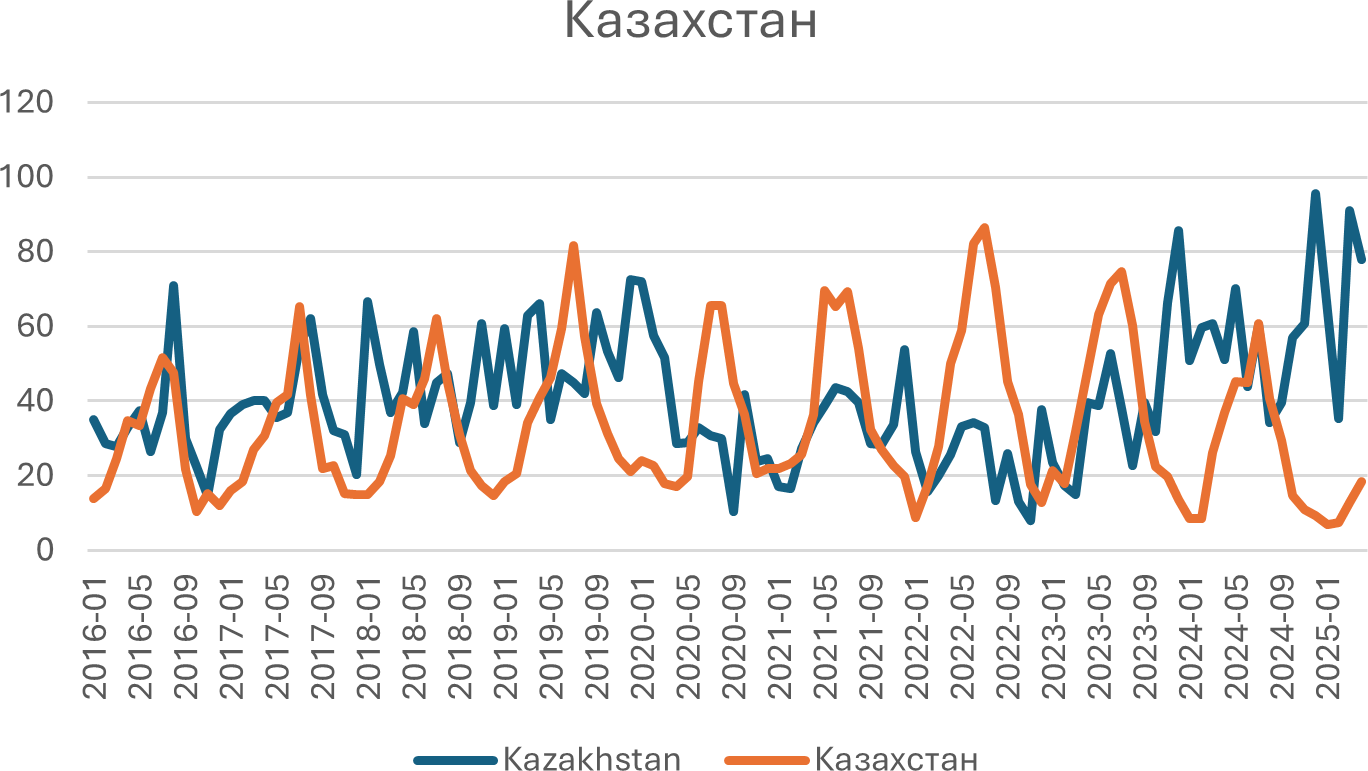
\includegraphics[width=0.7\textwidth]{media/ekon4/image7}
	\caption*{Рис.1 - Динамика агрегированных индексов интереса к направлению «Казахстан» (2016--2025)}
\end{figure}

\begin{multicols}{2}
В отличие от направления «Казахстан», где русскоязычные и англоязычные
индексы отражали принципиально разные типы интереса (локальные
достопримечательности против общей логистики), направления «Алматы»
(рис.2) и «Астана» (рис.3) демонстрируют высокую степень
согласованности индексов в допандемийный период (2016--2019). Это может
быть связано с тем, что оба города являются крупными центрами с
узнаваемыми брендами, как внутри страны, так и за её пределами.

Для Алматы в до пандемийные годы характерен устойчивый рост интереса по
обоим языковым сегментам, особенно в летние месяцы, что подтверждает
сезонную природу внутреннего туризма. В русскоязычном индексе сезонность
выражена сильнее, тогда как англоязычный интерес к городу остаётся более
сглаженным. Астана, в свою очередь, демонстрирует меньшую сезонность и
более ровную динамику, что, вероятно, связано с её восприятием как
административного и делового центра, а не как туристической дестинации в
привычном смысле.
\end{multicols}

\begin{figure}[H]
	\centering
	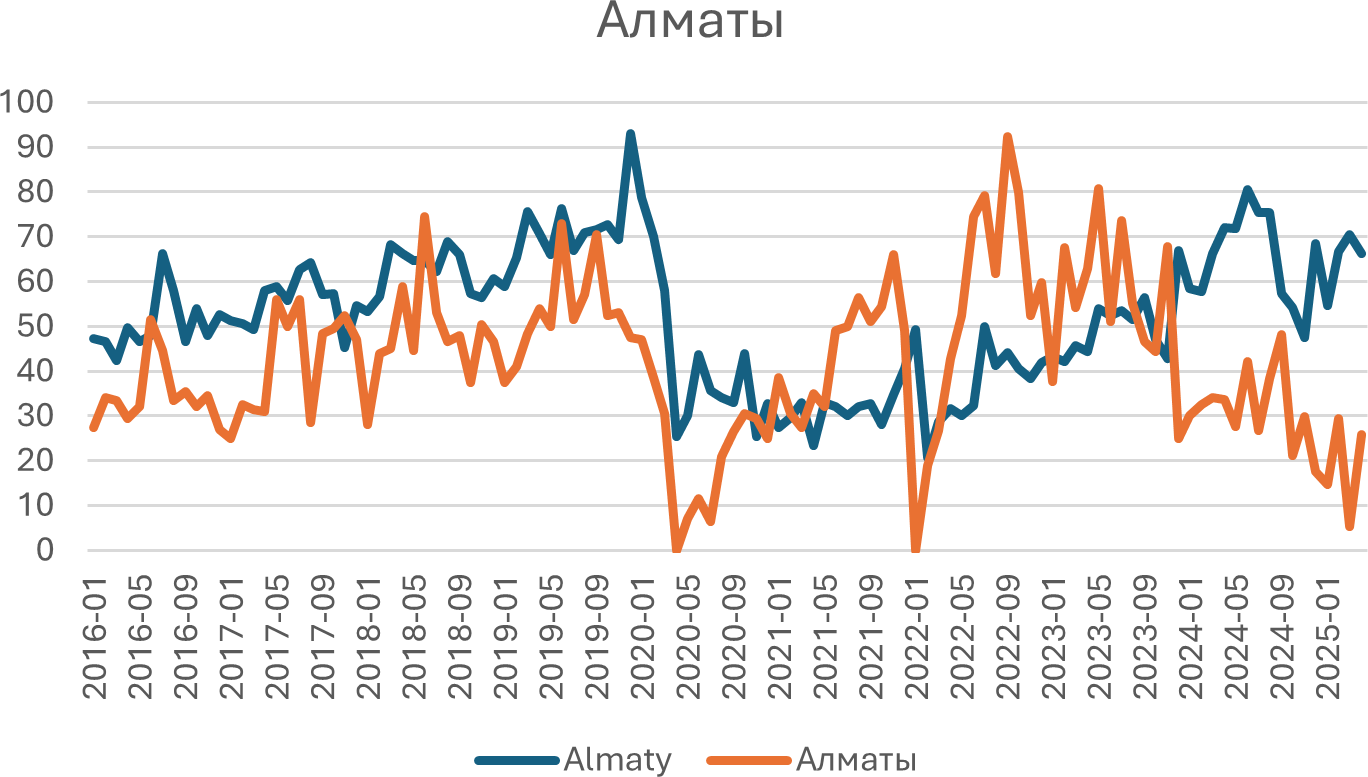
\includegraphics[width=0.7\textwidth]{media/ekon4/image8}
	\caption*{Рис.2 - Динамика агрегированных индексов интереса к направлению «Алматы» (2016--2025)}
\end{figure}
\begin{figure}[H]
	\centering
	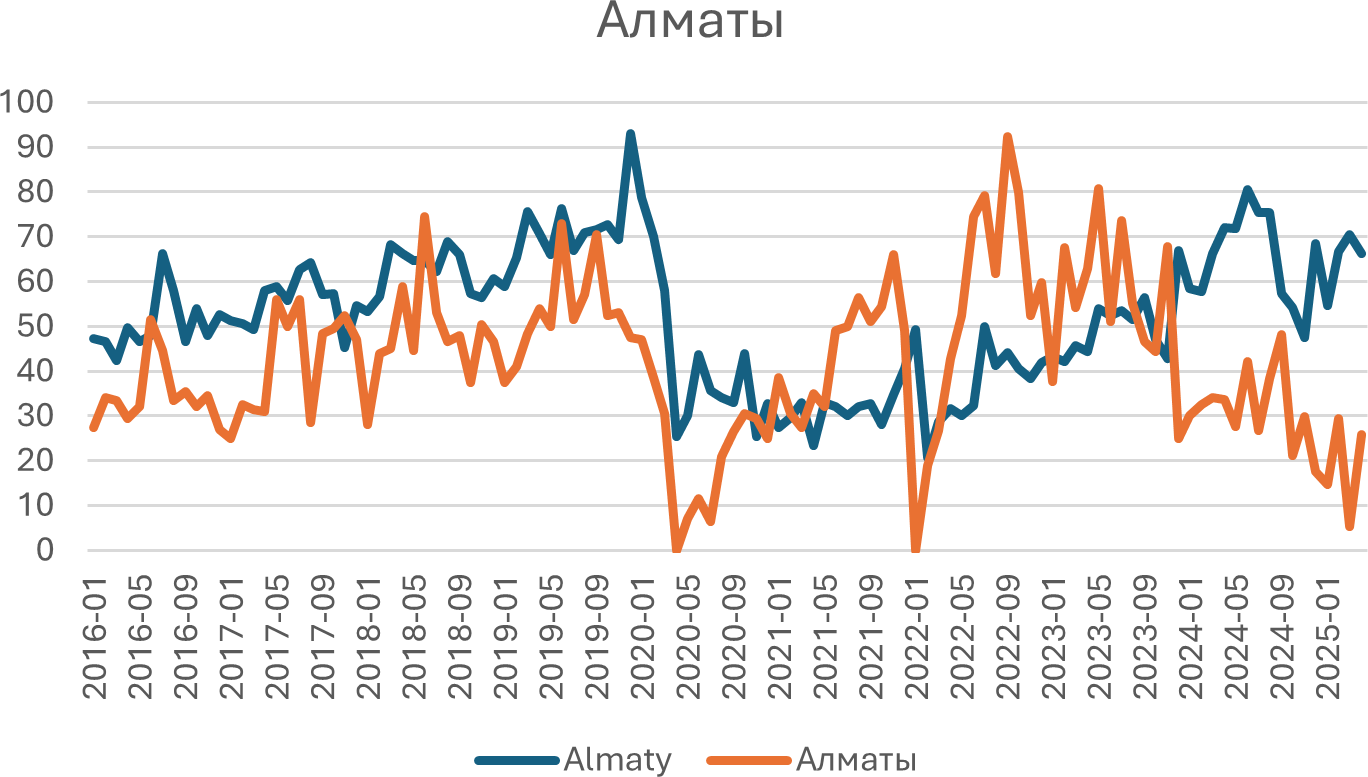
\includegraphics[width=0.7\textwidth]{media/ekon4/image8}
	\caption*{Рис.3 - Динамика агрегированных индексов интереса к направлению «Астана» (2016--2025)}
\end{figure}

\begin{multicols}{2}
Период 2020--2021 годов сопровождается резким снижением интереса к обоим
направлениям на фоне пандемии COVID-19. Однако восстановление происходит
с разной динамикой: для Алматы характерны выраженные сезонные всплески в
2022--2023 годах (особенно в русскоязычном сегменте), в то время как
англоязычный интерес к Астане восстанавливается более медленно, но
стабильно. Возможно, часть всплесков интереса к столице в 2022 году в
русскоязычном сегменте связана с внешнеполитическими событиями и
миграцией, а не напрямую с туризмом.

Таким образом, внутренний интерес к Алматы носит преимущественно
рекреационный характер с ярко выраженной сезонностью, тогда как интерес
к Астане более деловой и менее подвержен сезонным колебаниям. Это
подчёркивает различия в позиционировании и восприятии городов внутри и
за пределами страны.

{\bfseries Выводы.} Целью настоящего исследования было определение
потенциала использования поисковых данных Google Trends для анализа
интереса к туристическим направлениям в Казахстане. В качестве объекта
исследования рассматривался туристический спрос в Республике Казахстан,
а предметом --- поисковая активность в Google как отражение цифрового
поведения потенциальных туристов. Методологическая основа включала отбор
и фильтрацию 240 поисковых запросов, их агрегирование, корреляционный
анализ и последующее формирование индексов интереса к трем направлениям:
Алматы, Астана и Казахстан в целом, с учётом различий между
русскоязычной и англоязычной аудиторией.

Результаты анализа показали, что только 21 запрос соответствовал
критериям стабильности и согласованности. Это подчёркивает
ограниченность универсального применения Google Trends в региональных
исследованиях и необходимость тщательной предварительной фильтрации
данных. Среди отобранных запросов преобладали формулировки, связанные не
с достопримечательностями, а с процессом поездки (аэропорт, авиабилеты,
размещение), особенно в англоязычных группах, что может
свидетельствовать о преобладании делового туризма или логистически
ориентированного интереса со стороны международной аудитории.

Анализ индексов показал выраженные сезонные пики в русскоязычных
запросах по направлениям «Казахстан» и «Алматы», что соответствует
модели внутреннего рекреационного туризма. Напротив, интерес к Астане
отличался большей стабильностью и меньшей подверженностью сезонным
колебаниям, что может быть связано с её деловым и административным
статусом. Также выявлена разница в восприятии направления «Казахстан» в
зависимости от языка: англоязычные запросы фокусируются на поездке в
страну в целом, тогда как русскоязычные --- на отдельных природных
локациях.

Таким образом, полученные результаты подтверждают исходную гипотезу о
том, что поисковая активность в Google может отражать поведенческие
паттерны, связанные с туристическим спросом, особенно при соблюдении
корректной методики отбора и агрегации данных. В то же время применение
Google Trends в условиях Казахстана требует адаптации и осторожной
интерпретации из-за высокой чувствительности инструмента к формулировке
запросов и языковым аспектам.

Перспективы дальнейших исследований включают:

- расширение анализа за счёт включения казахоязычных запросов в рамках
локализованной выборки;

- формирование тематических подгрупп (например, экотуризм, медицинский
туризм);

- сопоставление цифрового интереса с фактической статистикой
туристических потоков (по возможности --- в помесячной динамике);

- разработку индексов, интегрирующих поисковые данные с социальными
медиа и системой бронирований.

- проведение регрессионного анализа для построения моделей
прогнозирования туристического спроса на основе цифровых индикаторов
--- при наличии соответствующей статистики.

Результаты исследования могут быть использованы как основа для
разработки инструментов мониторинга цифрового интереса к туристическим
направлениям, а также для оценки эффективности мероприятий по
продвижению туризма в Казахстане на национальном и региональном уровнях.
\end{multicols}

\begin{center}
{\bfseries Литература}
\end{center}

\begin{references}
1. Bokelmann B., Lessmann S. Spurious patterns in Google Trends data: An
analysis of the effects on tourism demand forecasting in Germany //
Tourism Management. -2019. -Vol.75. P. -1-12.
\href{https://doi.org/10.1016/j.tourman.2019.04.015}{DOI\\
10.1016/j.tourman.2019.04.015}

2. Cebrián E., Domenech J. Is it possible for Google Trends to forecast
rural tourism? The situation in Spain // Journal of Tourism Management
Research. -- 2024. -- Vol.11 (2). -- P.302-312.
\href{https://doi.org/10.18488/31.v11i2.3986}{DOI\\
10.18488/31.v11i2.3986}.

3. Грибок М. В., Горбунова Т. Ю. Сервис Google Trends как источник данных
для исследования ментальных связей между регионами России // Геополитика
и экогеодинамика регионов. - 2019. - № 3. - C/256-262

4. Федорченко С. Н. Политический анализ через оптику Google Trends (кейсы
Италии, США, России, Германии и Мексики) //Журнал политических
исследований. - 2019. -T.3 (4). С.142-156.

5. Соколов С.В. Применение веб-аналитического инструментария Google
Trends в социогуманитарных и библиотековедческих исследованиях.
Библиосфера.2018. - № 4:3-9.
\href{https://doi.org/10.20913/1815-3186-2018-4-3-9}{DOI
10.20913/1815-3186-2018-4-3-9}.

6. France C., Shi Y. Aggregating Google Trends: Multivariate Testing and
Analysis // Social Science Computer Review. - 2018.- Vol.36(4).- P.
460-475. DOI
\href{http://dx.doi.org/10.48550/arXiv.1712.03152}{10.48550/arXiv.1712.03152}.

7. Onder I. Forecasting tourism demand with Google Trends: Accuracy
comparison of countries versus cities // International Journal of
Tourism Research. - 2017.-Vol.19(6). - P.671682.
\href{https://doi.org/10.1002/jtr.2137}{DOI 10.1002/jtr.2137}.

8. Dinis G., Breda Z., Costa C., Pacheco O. Google Trends in tourism and
hospitality research: A systematic literature review // Journal of
Hospitality and Tourism Technology.- 2019. - Vol.10(4). -P.807-822.
DOI
\href{http://dx.doi.org/10.1108/JHTT-08-2018-0086}{10.1108/JHTT-08-2018-0086}.

9. Hasyyati A. N., Indriani R., Lestari T. K. Predicting Tourism Demand
in Indonesia Using Google Trends Data.-arXiv:2211.13938- 2022. DOI
10.48550/arXiv.2211.13938

10. Fitriani Y., Setiawan A. A. Predicting Tourism Demand in Indonesia
Using Google Trends Data // Indonesian Journal of
Geography.-2021.-Vol.53(3).-P.422-431.
\href{https://doi.org/10.48550/arXiv.2211.13938}{DOI
10.48550/arXiv.2211.13938}.
\end{references}

\begin{center}
{\bfseries References}
\end{center}

\begin{references}
1. Bokelmann B., Lessmann S. Spurious patterns in Google Trends data: An
analysis of the effects on tourism demand forecasting in Germany //
Tourism Management. -2019. -Vol.75. P. -1-12.
\href{https://doi.org/10.1016/j.tourman.2019.04.015}{DOI\\
10.1016/j.tourman.2019.04.015}

2. Cebrián E., Domenech J. Is it possible for Google Trends to forecast
rural tourism? The situation in Spain // Journal of Tourism Management
Research. - 2024. - Vol.11 (2). -P.302-312.
\href{https://doi.org/10.18488/31.v11i2.3986}{DOI\\
10.18488/31.v11i2.3986}

3. Gribok M. V., Gorbunova T. Ju. Servis Google Trends kak istochnik
dannyh dlja issledovanija mental' nyh svjazej mezhdu
regionami Rossii // Geopolitika i jekogeodinamika regionov. - 2019. - №
3. - C.256-262.{[}in Russian{]}

4. Fedorchenko S. N. Politicheskij analiz cherez optiku Google Trends
(kejsy Italii, SShA, Rossii, Germanii i Meksiki) //Zhurnal politicheskih
issledovanij. - 2019. -T.3 (4). S.142-156.{[}in Russian{]}

5. Sokolov S.V. Primenenie veb-analiticheskogo instrumentarija Google
Trends v sociogumanitarnyh i bibliotekovedcheskih issledovanijah.
Bibliosfera.2018. - № 4:3-9. DOI 10.20913/1815-3186-2018-4-3-9.{[}in
Russian{]}

6. France C., Shi Y. Aggregating Google Trends: Multivariate Testing and
Analysis // Social Science Computer Review. - 2018.- Vol.36(4).- P.
460-475. DOI
\href{http://dx.doi.org/10.48550/arXiv.1712.03152}{10.48550/arXiv.1712.03152}.

7. Onder I. Forecasting tourism demand with Google Trends: Accuracy
comparison of countries versus cities // International Journal of
Tourism Research. - 2017.-Vol.19(6). - P.671682.
\href{https://doi.org/10.1002/jtr.2137}{DOI 10.1002/jtr.2137}.

8. Dinis G., Breda Z., Costa C., Pacheco O. Google Trends in tourism and
hospitality research: A systematic literature review // Journal of
Hospitality and Tourism Technology.- 2019. - Vol.10(4). -P.807-822.
DOI
\href{http://dx.doi.org/10.1108/JHTT-08-2018-0086}{10.1108/JHTT-08-2018-0086}.

9. Hasyyati A. N., Indriani R., Lestari T. K. Predicting Tourism Demand
in Indonesia Using Google Trends Data.-arXiv:2211.13938- 2022. DOI
10.48550/arXiv.2211.13938

10. Fitriani Y., Setiawan A. A. Predicting Tourism Demand in Indonesia
Using Google Trends Data // Indonesian Journal of
Geography.-2021.-Vol.53(3).-P.422-431.
\href{https://doi.org/10.48550/arXiv.2211.13938}{DOI
10.48550/arXiv.2211.13938}.
\end{references}

\begin{authorinfo}
\emph{{\bfseries Сведения об авторе}}

Идрышов М. Б.- PhD student/докторант, лектор, НАО
«Восточно-Казахстанский университет им. С.Аманжолова», Усть-Каменогорск,
Казахстан, e-mail: immakhambet@gmail.com.

\emph{{\bfseries Information about the author}}

Idryshov M.B.- PhD student, Lecturer, S. Amanzholov East Kazakhstan
University, Ust-Kamenogorsk, Kazakhstan, e-mail: immakhambet@gmail.com.
\end{authorinfo}
